\newpage


\section{Przegląd literatury}
\label{sec:literature}

\subsection{Istniejące metody partycjonowania grafów}

1. Rozbudowany podział metod został zaproponowany przez autorów artykułu - \cite{metis}
oraz \cite{1364754}
Zgodnie z ich analizą metody dzielimy na:
\begin{itemize}
    \item spektralne,
    \item rekursywne,
    \item geometryczne,
    \item wielopoziomowe.
\end{itemize}

\subsubsection{Metody spektralne}
\begin{wrapfigure}{r}{0.35\textwidth}
    \vspace{-4mm}
    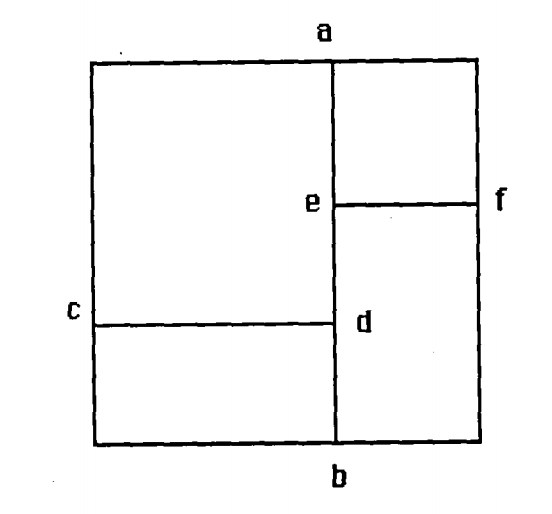
\includegraphics[width=\linewidth]{images/recursive}
    \caption{Przedstawia partycjonowanie rekursywne na głębokości wynoszącej 2. Linia partycjonowania a-b, która została stworzona
    przez partycjonowanie poziomu 1 jest podzielona na 3 segmenty przez dwie linie partycjonowania poziomu drugiego:
    c-d, e-f. Źródło: \cite{recursive}}
    \label{im:recursive_partitioning}
\end{wrapfigure}
Partycjonowanie spektralne daje dobre rezultaty i jest metodą w miarę często używaną
\cite{10.1137/0611030, 10.5555/147877.147902, improved_spectral}.
Metoda \cite{10.1137/0611030} pokazuje algebraiczne podejście do obliczania separatorów wierzchołków - dolne granice
rozmiarów separatorów można uzyskać w postaci wartości własnych macierzy Laplace'a związanej z grafem.
Wektory własne Laplace'a (!!!) grafów siatkowych (!!!) można obliczyć z iloczynów Kroneckera (!!!) obejmujących wektory własne grafów typu
ścieżka, a te wektory własne mogą być użyte do obliczania separatorów w grafach siatkowych.
Artykuł \cite{10.5555/147877.147902} opisuje algorytm spectral nested dissection (SND) (!!!).
Algorytm ten za pomocą znajomości spektralnych właściwości macierzy Laplacian (org. Laplacian matrix) (!!!) oblicza separatory w grafie.
Artykuł \cite{improved_spectral} mówi o nowatorskim rozwinięciu metody spektralnej pod kątem umożliwienia podziału
obliczeń na cztery bądź osiem części na każdym etapie rekursywnej dekompozycji.
Są to jednak wszystko metody kosztowne z racji na
obliczanie wektorowa własnego odpowiadającego drugiej najmniejszej wartości własnej (Fielder wektor).
Istnieją udane próby ulepszenia czasu wykonania tych metod, które polegają na liczeniu Fielder wektora poprzez
algorytm wielopoziomowy - MSB \cite{fast_multilevel}. Jednak nawet te metody wciąż charakteryzują się wysoką złożonością.

\subsubsection{Metody rekursywne}

Są to metody często prostsze w implementacji, jednak nie sprawdzają się tak dobrze w kontekście bardziej
skomplikowanych problemów głównie ze względu na to, że mają zachłanną naturę.
Ponadto wykorzystanie takich algorytmów w kontekście niepodzielnych obszarów nie zdaje egzaminu,
ze względu na ich specyfikę. Podejście do partycjonowania zakładające dzielenie grafu na coraz mniejsze
części sprawia, że nie jesteśmy w stanie uwzględniać części niepodzielnych, lub rozwiązanie tego problemu byłoby skomplikowane.
Przykład - dzielimy siatkę na 4 części. Można sobie wyobrazić sytuację, kiedy obszar niepodzielny zajmuje 50\% całej siatki.
Po pierwszej turze rekursywnego algorytmu mamy dwie partycje, każda zajmująca 50\% powierzchni. Chcielibyśmy podzielić
każdą z nich na dwie części, natomiast nie jesteśmy w stanie tego zrobić ponieważ jedna z nich jest w całości obszarem
niepodzielnym.
Metoda \cite{recursive} zakłada żę dzielimy siatkę na liczbę obszarów,
która jest równa potędze liczby dwa. Ta metoda potrafi także dzielić siatkę wedle możliwości obliczeniowych
poszczególnych rdzeni procesora. Czasami metody rekursywne są implementowane jako faza metod
bisekcji spektralnej \cite{10.1137/0611030}. Przykłady działania partycjonowania rekursywnego przedstawione są na rysunkach
\ref{im:recursive_partitioning} oraz \ref{im:rec_partitioning}.


\begin{figure}[h]
    \centering
    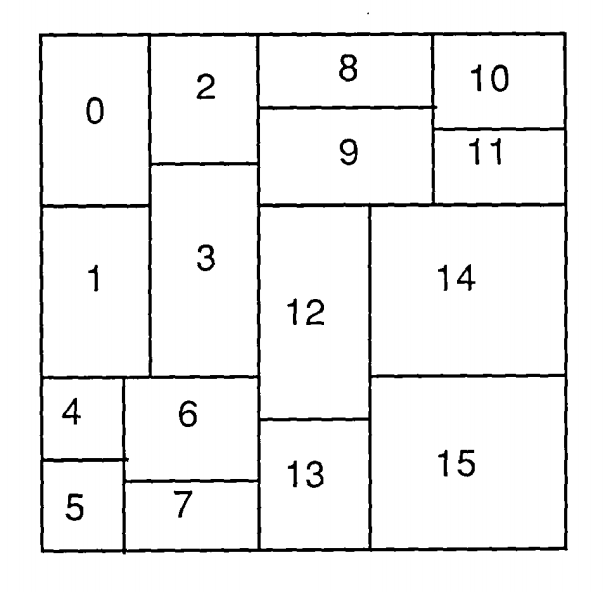
\includegraphics[width=0.5\linewidth]{images/recursive-part}
    \caption{Metoda rekursywna - binarna dekompozycja dla 16 procesorów. Najpierw tworzone jest wertykalne cięcie,
        które gwarantuje, że prawy i lewy obszar
    zawiera połowę pracy do wykonania (lub takie, które jest jak najbliżej takiego podziału). Jeśli dostępne
    są 4 procesory to każdy z dwóch segmentów partycjonowany jest horyzontalną linią, która spełnia te same założenia
    jak ta dla pierwszego wertykalnego cięcia. Procedura jest kontynuowana na zmianę wykorzystując wertykalne i
    horyzontalne cięcie aż do otrzymania podziału na oczekiwaną liczby obszarów. Źródło: \cite{recursive}}
    \label{im:rec_partitioning}
\end{figure}

\newpage

\subsubsection{Metody geometryczne}

\begin{wrapfigure}{r}{0.41\textwidth}
    \vspace{-4mm}
    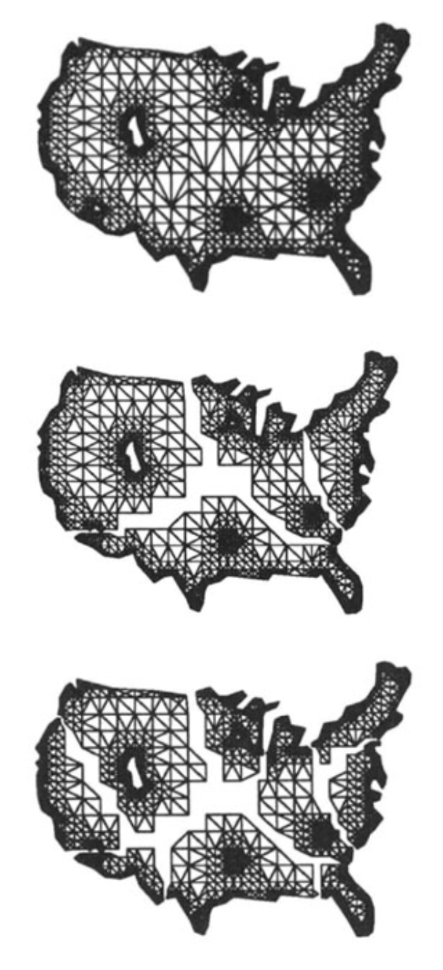
\includegraphics[width=\linewidth]{images/recursive-partitioning}
    \caption{Rekursywne partycjonowanie mapy USA - pierwszy obrazek od góry - za pomocą algorytmu numer 5 z artykułu \cite{MiTeThVa93},
        strona 76. Dwa następne obrazki prezentują rezultat. Najpierw używane są geometryczne dane do obliczenia
        ''continuous separator'' (!!!), następnie znajdowany jest ''vertex separator'' (!!!).}
\end{wrapfigure}


Inną klasą metod są metody geometryczne
\cite{Miller1994ACP, Raghavan93lineand, 185417, MiTeThVa93, NourOmid1987SolvingFE}.
Ich cechą charakterystyczną jest szybki czas wykonania, natomiast gorsze rezultaty podziału.
Najlepsze wyniki spośród wyżej wymienionych metod prezentują \cite{185417, MiTeThVa93}.
W artykule \cite{185417} zaproponowane klasę grafów zwaną k-overlap graphs (!!!). Istnienie
separatora granicznego (separator bound) (!!!) jest udowodniony dla grafów k-overlap osadzonych (embedded) (!!!) w d wymiarach. Wyniki w tym
artykule unifikują kilka wcześniejszych wyników dla separatorów.
Separatory graniczne są obliczane w czasie liniowym (randomized linear-time) (!!!).
Jeśli mamy K separatorów dla grafu o N wierzchołkach oznacza to, że istnieje podzbiór wierzchołków o wielkości K,
których usunięcie spowoduje powstanie dwóch komponentów o mniej więcej podobnym rozmiarze.
W artykule \cite{MiTeThVa93} opisano efektywną metodę partycjonowania siatek niestrukturalnych, która występują w metodach
elementów skończonych (!!!) i różnic skończonych (!!!). Podejście to wykorzystuję strukturę geometryczną danej siatki i znajduje
dobre partycjonowanie w czasie \(O(n)\). Można je aplikować do siatek w dwóch i trzech wymiarach. Ma zastosowanie
w wydajnych algorytmach sekwencyjnych i równoległych do rozwiązywania rozbudowanych problemów (large-scale problems)
w obliczeniach naukowych.
Charakterystyką metod geometrycznych jest to, że z powodu losowej natury wymagane jest wielokrotne użycie algorytmu
(od 5 do 50 razy) aby uzyskać wynik porównywalny z metodami spektralnymi.
Wielokrotnie wywołanie zwiększa czas otrzymywania rezultatu, natomiast jest
on wciąż niższy od metod spektralnych. Metody geometryczne są aplikowalne tylko w przypadku kiedy dostępne
są współrzędne wszystkich wierzchołków w grafie. Dla wielu dziedzin problemów (programowanie liniowe, VLSI),
nie otrzymujemy współrzędnych wraz z grafem. Istnieją algorytmy, które są w stanie obliczyć współrzędne dla
wierzchołków grafu \cite{Chan95geometricspectral} wykorzystując metody spektralne ale są bardzo kosztowne i dominują czas potrzebny
na samo partycjonowanie grafu.

\newpage

\subsubsection{Metody wielopoziomowe}

\begin{figure}[h]
    \centering
    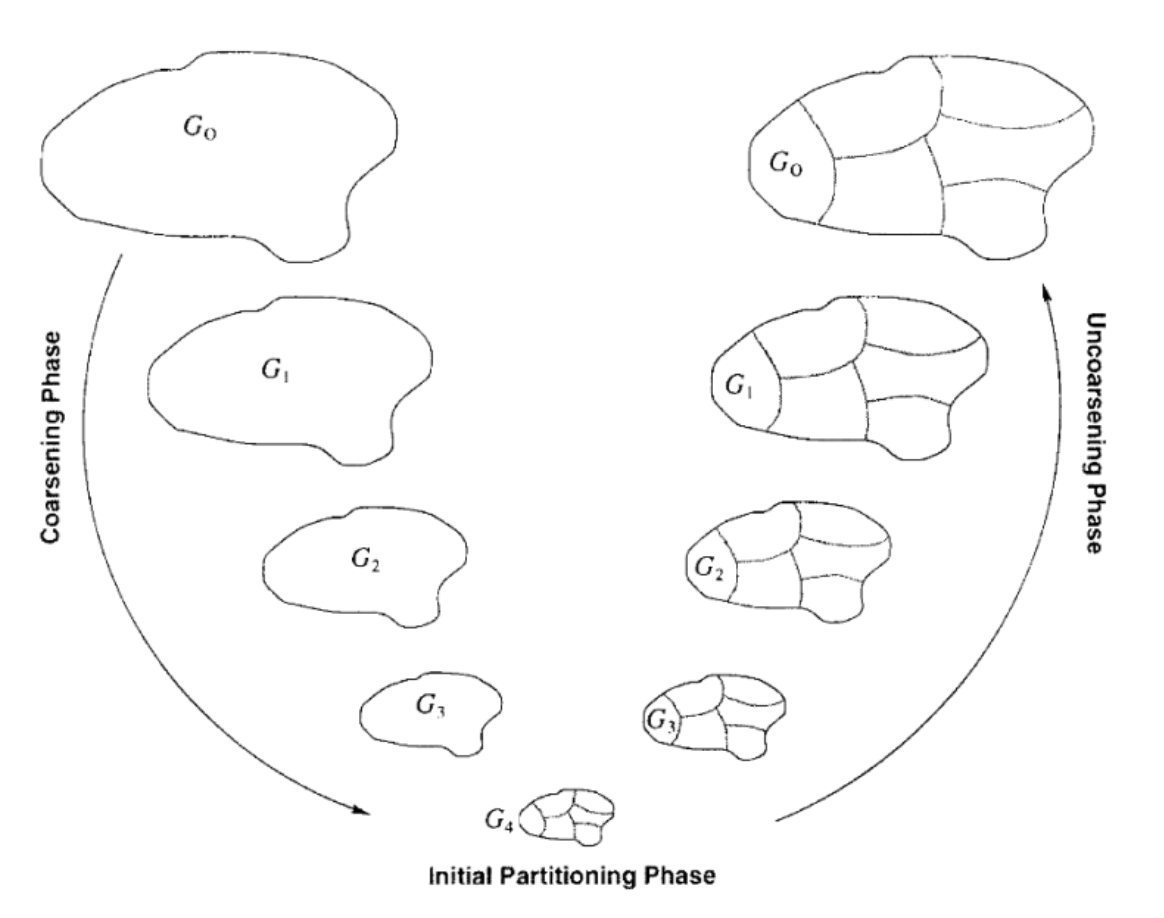
\includegraphics[width=\linewidth]{images/coarsening}
    \caption{Wielopoziomowe partycjonowanie grafu przedstawiające fazę zmniejszania grafu, następnie przypisanie
    partycji na zmniejszonym grafie, na końcu przywrócenie grafu do początkowej wielkości.
    Źródło: \cite{KARYPIS199896}.}
    \label{im:multilevel_partitioning}
\end{figure}

\cite{metis, jostle, Bui1993AHF, 103500, 185177, 279334, inproceedings, 129970, 10.1145/165939.165942}
- cechą charakterystyczną tego podejścia jest redukcja
wielkości grafu poprzez łączenie wierzchołków i krawędzi, następnie dzielenie zmniejszonego grafu na partycje, ostatnią fazą
jest przywrócenie początkowego grafu zachowując podział. Często graf zmniejszany jest aż liczba wierzchołków nie osiągnie
liczby partycji, którą chcemy otrzymać \cite{1364754}, a fazie przywracania grafu do początkowej wielkości towarzyszy
algorytm, którego celem jest ulepszanie podziału \cite{article, 10.5555/800263.809204}. Algorytm ten, bazując na zmniejszonym
grafie, niesie za sobą niższy koszt obliczeniowy. Jego działanie polega na zmniejszaniu długości granic pomiędzy partycjami
z jednoczesnym zachowaniem ich wielkości. Na tym etapie może także zostać dodana faza balansowania, która stopniowo zmniejsza różnice
w wielkości pól pomiędzy obszarami. Metody te zostały stworzone z myślą o zmniejszeniu czasu
patrycjonowania kosztem jego jakości. Obecnie dają jednak bardzo dobre rezultaty również w kwestii jakości podziału.
Późniejsze prace w dziedzinie tych algorytmów pokazały, że dają one lepsze rezultaty niż metody spektralne \cite{metis}.
Biblioteki jak Party \cite{1364754}, Metis \cite{metis}, Jostle \cite{jostle}, Chaco \cite{inproceedings},
dające state-of-the-art wyniki w kwestii jakości partycjonowania najczęściej bazują na schemacie wielopoziomowym
\cite{inproceedings}.

\newpage

\subsection{Porównanie istniejących metod wielopoziomowych}

\begin{wrapfigure}{r}{0.6\textwidth}
    \vspace{-4mm}
    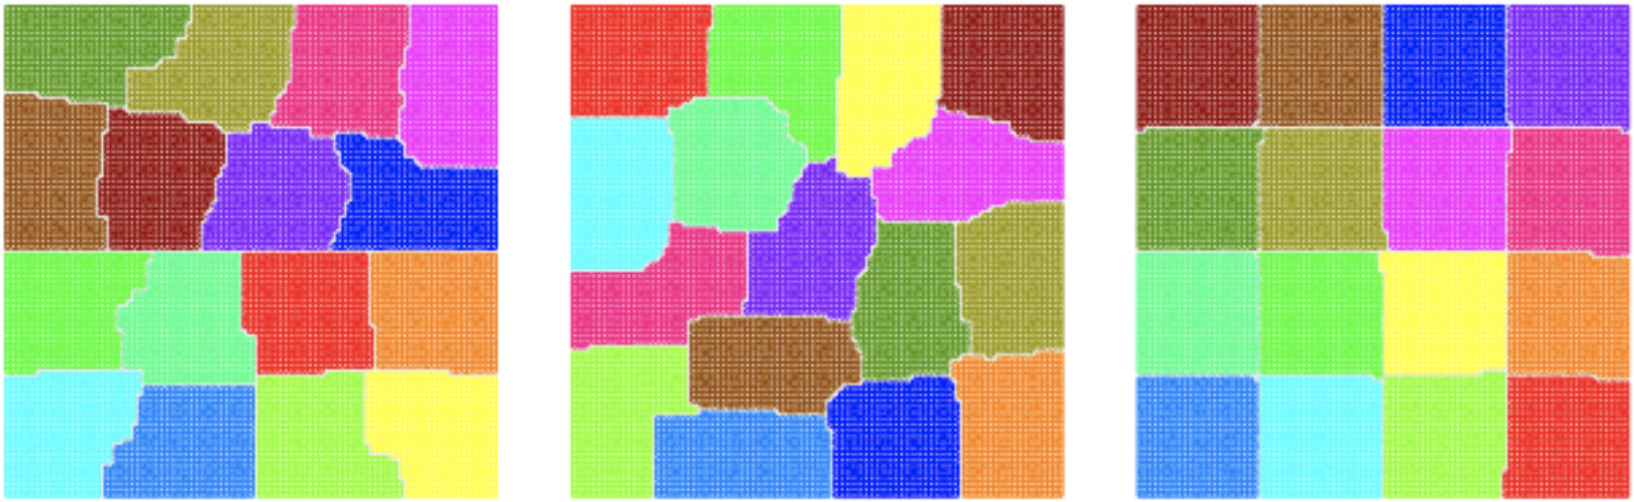
\includegraphics[width=\linewidth]{images/libraries-comparision}
    \caption{Partycjonowanie siatki 100x100 na 16 obszarów. Od lewej - pmetis \cite{metis} uzyskuje edge-cut wynoszący
    688, następnie Jostle \cite{jostle} z wynikiem 695 oraz Party \cite{1364754} z wynikiem 615. Źródło: \cite{1364754}.}
    \label{im:partitioning_results}
\end{wrapfigure}

Wszystkie wyżej wymienione metody nie biorą pod uwagę problemu obszarów niepodzielnych oraz obszarów wyłączonych z obliczeń.
W związku z tym moim zadaniem było znalezienie metody dającej możliwie najlepsze rezultaty w zakresie partycjonowania grafów oraz
dostosowanie jej do wyżej wymienionych rozszerzeń problemu partycjonowania.

Metody wielopoziomowe były najlepszym wyborem, z racji na to, że gwarantowały najlepsze wyniki partycjonowania.
Przykładów metod wielopoziomowych było bardzo dużo \cite{metis, jostle, Bui1993AHF, 103500, 185177, 279334, inproceedings, 129970, 10.1145/165939.165942},
jednak skupiłem się głównie na tych, które dawały wyniki state-of-the-art. Były to biblioteki:
Party \cite{1364754}, Metis \cite{metis}, Jostle \cite{jostle}, Chaco \cite{inproceedings}.

Do zmniejszenia grafu stosowane są różne warianty matching algorithm (algorytm do budowania skojarzeń w grafie).
Porównanie większości z nich można znaleźć tutaj \cite{Analysis}.
Przykładowo biblioteka Jones oraz Bui \cite{Bui1993AHF} używam random weighted matching, natomiast Party \cite{1364754}
stosuje LAM matching \cite{weighted_maching}.
Ze względu na wymagania co do złożoności obliczeniowej wszystkie metody używają heurystyk.
Wszystkie z tych metod zmniejszają graf, jednak tylko Jostle i Party zmniejsza graf
aż do otrzymania liczby wierzchołków równej liczbie partycji, na które chcemy podzielić wejściowy graf.
Dzięki temu metoda partycjonowania, działająca na najmniejszym możliwym grafie, jest dużo prostsza niż w pozostałych metodach.
Kiedy graf jest zmniejszony, wierzchołki są przyporządkowywane do partycji a informacja na temat partycji jest propagowana
do wierzchołków na wyższych poziomach zgodnie z partycją ich reprezentantów na najniższym poziomie. Ten proces prowadzi
do partycjonowania początkowego grafu. Faza zmniejszania grafu jest ponadto stosunkowo łatwa do zrównoleglenia \cite{KARYPIS199871}.
Fazą, która nie podlega zrównolegleniu jest faza ulepszania istniejącego podziału.
Najczęściej bazuje ona na metodzie Fiduccia-Mattheysesa \cite{10.5555/800263.809204},
która jest zoptymalizowaną pod kątem czasu działania heurystyką Kerninghan-Lin (KL) \cite{6771089}.
W przeciwieństwie do Metis i Jostle, faza ulepszenia partycjonowania używana przez biblioteke Party bazuje na metodzie
Helpful-Sets (HS). Heurystyka Helpful-Set wywodzi się z obserwacji teoretycznych wykorzystywanych do znajdowania górnych
granic szerokości bisekcji grafów regularnych \cite{10.1007/3-540-54345-7_64, MONIEN2006475}.
Szerokość bisekcji to minimalna liczba krawędzi, która musi zostać usunięta w celu podzielenia grafu na
dwie równej wielkości części, lub różniące się wielkością o maksymalnie jeden wierzchołek.
Party otrzymuje bardzo dobre wyniki stosując tę metodę \cite{10.1007/3-540-44842-X_6}, często uzyskując mniejszą długość
granic pomiędzy obszarami niż Metis czy Jostle, jednocześnie jest tylko trochę bardziej kosztowna obliczeniowo.
Heurystyka Helpful-Sets jest metodą bazującą na wyszukiwaniu lokalnym. Zaczynając od początkowej bisekcji \(\pi\) dąży
do zminimalizowania długości granicy za pomocą lokalnie wprowadzanych zmian. Najważniejsza różnica względem metody KL
polega na tym że KL przemieszcza tylko pojedyncze wierzchołki, natomiast HS zbiory wierzchołków. Zarówno Party, Metis
jak i Jostle pozwalają na małe nierówności w kwestii wielkości obszarów co przekłada się na mniejsze długości granic,
szczególnie na głębszych poziomach, kiedy przemieszczane są wierzchołki o dużych wagach - ciężko wtedy o otrzymanie
idealnie równych obszarów.

Biblioteka Party \cite{1364754} okazała się dawać najlepsze rezultaty w porównaniu do innych bibliotek dających wyniki
state-of-the-art. Szczególną własnością Party była znacznie niższa długość granic w porównaniu do pozostałych bibliotek
[Rysunek \ref{im:partitioning_results}], co było bardzo ważne dla mojej pracy. Dlatego to właśnie metodę z biblioteki
Party zdecydowałem się modyfikować pod kątem obszarów niepodzielnych oraz obszarów wyłączonych z obliczeń.
